\chapter{Arquitecturas de \textit{software}}

Según \cite{taylorSoftwareArchitectureFoundations2009}, la {\bf arquitectura de un sistema \textit{software}} es el conjunto de todas las decisiones de diseño principales que se toman durante la vida del sistema, aquellas que sientan las bases del desarrollo. \textcolor{red}{Se podría establecer un simil con los planos de construcción de un edificio.} Estas decisiones no solo se toman durante su concepción, si no también durante su desarrollo y posterior evolución.

La arquitectura afecta a todos los apartados del sistema: su estructura, funcionalidad, la implementación\dots Por ejemplo, una decisión de diseño principal que se suele tomar en las fases tempranas del desarrollo es la elección de la topología para la solución. Optar por desarrollar un servicio monolítico o una arquitectura basada en microservicios va a condicionar prácticamente todo el desarrollo. Desde el diseño, la implementación, el testeo, y sobre todo, el despliegue y operación. \textcolor{red}{Por tanto, es vital dedicar tiempo para definir la arquitectura en base a las necesidades de nuestro sistema.}

\section{Decisiones principales de diseño}

Las decisiones principales de diseño normalmente se resumen en comparativas entre distintas alternativas, cada una de ellas con sus ventajas e inconvenientes. Con el paso del tiempo, y con el avance del desarrollo, estas elecciones comienzan a asentarse, y se vuelven más dificiles de cambiar o rectificar.

Pueden tomarse en base a distintos criterios. Entre ellos podemos destacar: [Citation needed]

    \begin{itemize}
        \item \textbf{Requisitos del sistema:} a partir del dominio y las necesidades de nuestros usuarios, podemos deducir: la funcionalidad a implementar, las restricciones que debemos respetar y otras propiedades que debe poseer el sistema.

        \item \textbf{Arquitectura actual:} las decisiones tomadas previamente también condicionan las elecciones que se tomen más adelante. Cuanto más avanza el desarrollo, más se asientan las decisiones previas, y más dificil es rectificarlas.

        \item \textbf{Experiencia previa:} del desarrollo de este u otros sistemas. Podemos obtener métricas del funcionamiento y uso de nuestro sistema para informar decisiones futuras. \textcolor{red}{[Cita devops]}
    \end{itemize}

\section{Componentes de una arquitectura}

Según el estándar IEEE 42010-2011 \cite{ieeeStandard420102011Systems2011}, la arquitectura de un sistema es "\textit{un conjunto de conceptos o propiedades fundamentales, personificados por sus elementos, sus relaciones, y los principios que guían su diseño y evolución}". Nos provee de un marco de referencia común, de decisiones que nos nos provee con un vocabulario común, que nos permite describir sistemas

Por tanto, podemos describirla usando tres conceptos: \cite{perryFoundationsStudySoftware1992}

    \begin{itemize}
        \item \textbf{Componentes:} Son las piezas fundamentales que componen el sistema. Implementan la funcionalidad de la aplicación. Se utilizan para describir \textit{qué} partes conforman el sistema. Por ejemplo: un módulo, un servicio web...

        \item \textbf{Forma:} El conjunto de propiedades y relaciones entre los elementos o el entorno de operación. Describe \textit{cómo} está organizado el sistema. Por ejemplo: un servicio contacta con otro a través de una API.

        \item \textbf{Justificación:} Razonamiento o motivación de las decisiones que se han tomado. Responden al \textit{por qué} algo se hace de determinada forma. Normalmente no pueden deducirse a partir de los elementos y la forma, por lo que es necesario describirlos.

    \end{itemize}

\textcolor{red}{La arquitectura de un sistema puede contar con diferentes vistas, según aquel aspecto que deseemos resaltar. Por ejemplo, puede interesarnos más la interacción entre los componentes. O cosas por el estilo.}

Durante el diseño, para lidiar con la complejidad que pudiera alcanzar el sistema, solemos recurrir a descomponerlos usando diseños modulares: sistemas compuestos por unidades de funcionalidad que tienen una función específica. \cite{taylorSoftwareArchitectureFoundations2009} Estos elementos funcionales son los componentes. Dependiendo de las características de nuestro sistema, pueden tomar distintas formas: módulos dentro un mismo proceso, servicios distribuidos, etc.

Como hemos comentado antes, un sistema está conformado por \textbf{componentes} que implementan la funcionalidad de la aplicación. No suelen trabajar de forma aislada, si no que trabajan conjuntamente para realizar tareas más complejas. Por tanto, un aspecto clave es la integración y la interacción entre ellos. \cite{mehtaTaxonomySoftwareConnectors2000}

Para que dos o más componentes puedan interactuar, necesitamos definir un mecanismo de comunicación. Para ello, recurrimos a los \textbf{conectores}: se trata de elementos arquitectónicos que nos ayudan a diseñar y razonar sobre la comunicación entre componentes. Representan la transferencia de datos y de control entre componentes. En la figura \ref{fig:componentesEjemplo} mostramos una representación de la necesidad de comunicación entre dos componentes a través de un conector. No se ha especificado todavía ningún detalle sobre cómo se implementará. De esta forma, podemos estudiar la arquitectura y elegir los mecanismos adecuados para cada interacción del sistema. \cite{taylorSoftwareArchitectureFoundations2009}.

\begin{figure}[h!]
  \centering
  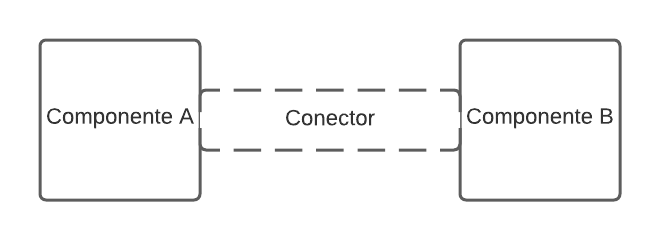
\includegraphics[scale=0.78]{02_arquitectura/images/conector}
  \caption{Ejemplo de comunicación de dos componentes a través de un conector.}
  \label{fig:componentesEjemplo}
\end{figure}

\textcolor{red}{A nivel de ¿diseño?}, los conectores están compuestos por uno o más \textbf{conductos} o canales de comunicación. A través de estos se lleva a cabo la comunicación entre los componentes. Hay una gran variedad de conductos posibles: comunicación interproceso, a través de la red, etc. Clasificamos los conectores según la complejidad de los canales que utilizan \cite{mehtaTaxonomySoftwareConnectors2000}:

\begin{itemize}
    \item \textbf{Conectores simples}: solo cuentan con un conducto, sin lógica asociada. Son conectores sencillos. Suelen estar ya implementados en los lenguajes de programación. Por ejemplo: una llamada a función en un programa o el sistema de entrada / salida de ficheros.

    \item \textbf{Conectores complejos}: cuentan con uno o más conductos. Se definen por composición a partir de múltiples conectores simples. Además, pueden contar con funcionalidad para manejar el flujo de datos y/o control. Suelen utilizarse importando \textit{frameworks} o librerias. Por ejemplo: un balanceador de carga que redirige peticiones a los nodos.
\end{itemize}

Por tanto, una vez hemos decidido que dos componentes deben comunicarse, es momento de evaluar cuál es el mecanismo de comunicación más adecuado. Para ello, podemos consultar la taxonomía de conectores de \cite{mehtaTaxonomySoftwareConnectors2000}. Basándonos en nuestros requisitos, la arquitectura ya definida, y los mecanismos de despliegue que queremos usar, elegimos el conector más adecuado.

Proxy o RMI

Abstraen al cliente de la lógica para establecer la conexión, el protocolo de comunicación, formato de los mensajes, etc

\subsection{Open API}

\begin{wrapfigure}{r}{0.35\linewidth}
  \vspace{15pt}
  
\includegraphics[scale=0.34]{02_arquitectura/images/openapi-logo}
  \centering
  \vspace{15pt}
\end{wrapfigure}

Para el desarrollo de este trabajo, hemos optado por utilizar conectores basados en APIs REST. Nos permitía utilizar mecanismos ya presentes en los microservicios que queríamos desarrollar, y que fueran más homogéneos.
Para facilitar la compatibilidad de los microservicios, y facilitar el desarrollo de nuevos microservicios, hemos decidido usar la especificación OpenAPI\footnote{Open API specification: \url{https://spec.openapis.org/oas/latest.html}}. Se trata de un estándar para describir APIs implementadas sobre el protocolo HTTP.

La principal ventaja que nos ofrecía OpenAPI era la posibilidad de generar código a partir de la especificación. Permite generar código tanto del cliente como del servidor. De esta forma, podíamos implementar nuestra API genérica en un lenguaje . En este caso, se decidió utilizar conjuntamente el lenguaje C\# junto con el framework ASP.NET Core, para implementar los microservicios iniciales.

A partir de estos microservicios, podemos exportar la especificación de OpenAPI, haciendo uso de los endpoints, atributos y comentarios. Por ejemplo, en este endpoint del servicio de monitorización, vemos cómo obtiene una propiedad del servicio de conocimiento.

Podemos observar cómo el método está decorado con atributos que describen el tipo de respuesta que produce, según el código de respuesta HTTP. Estos comentarios se utilizan en la generación de la especificación para obtener mejor implementación

Después, haciendo uso de las librerías de generación de código de OpenAP.
